\documentclass{article}
\usepackage[utf8]{inputenc}
\usepackage{geometry}
\usepackage{amsmath}
 \geometry{
 a4paper,
 total={170mm,257mm},
 left=20mm,
 top=20mm,
 }
 \usepackage{graphicx}
 \usepackage{titling}

 \title{Assignment \textbf{8} (Lecture 26-28)
}
\author{Syed Suhaib Ahmad}
\date{\today}
 
 \usepackage{fancyhdr}
\fancypagestyle{plain}{%  the preset of fancyhdr 
    \fancyhf{} % clear all header and footer fields
    
    \fancyfoot[C]{1}
    \fancyhead[L]{8.02x - Electricity and Magnetism}
    \fancyhead[R]{\theauthor}
}
\makeatletter
\def\@maketitle{%
  \newpage
  \null
  \vskip 1em%
  \begin{center}%
  \let \footnote \thanks
    {\LARGE \@title \par}%
    \vskip 1em%
    %{\large \@date}%
  \end{center}%
  \par
  \vskip 1em}
\makeatother

\usepackage{lipsum}  
%\usepackage{cmbright}

\begin{document}

\maketitle


\subsubsection*{Problem 8.1 - An $LRC$ Circuit}
A circuit contains self-inductance $L$ in series with a capacitor $C$ and a resistor $R$. This circuit is driven by an alternating voltage $V=V_0\sin\omega t$. We have $L=15\,$mH, $R=80\,\Omega$, $C=5\,\mu$F, and $V_0=40$ volts.
\begin{enumerate}
    \item[(a)]What is the resonance frequency, $\omega_0$?
    \item[(b)]Consider three separate cases for which $\omega=0.25\omega_0$, $\omega=\omega_0$, and $\omega=4\omega_0$ respectively. For each case, calculate the peak current $I_0$.
    \item[(c)]Find the energy $U_C(t)$ and the energy $U_L(t)$ stored, respectively, in the capacitor and in the inductor as a function of time for $\omega=\omega_0$.
\end{enumerate}
\textbf{Solution(a)}
\\
\\The formula for the resonance frequency can be easily determined from the expression for the amplitude of current in an $RLC$ circuit (when the inductive reactance cancels the capacitive reactance). Substituting the given values into the formula gives
\[\omega_0=\frac{1}{\sqrt{LC}}=\frac{1}{\sqrt{15\times10^{-3}\times5\times10^{-6}}}\approx3650\,\text{rad\,s}^{-1}.\]
\textbf{Solution(b)}
\\
\\Peak current is given by
\begin{equation}
    I_0=\frac{V_0}{\sqrt{R^2+\left(\omega L-\frac{1}{\omega C}\right)^2}}
\end{equation}
Thus, for each value of $\omega$ given in the problem, the peak current is given below.
\[\omega=0.25\omega_0\longrightarrow I_0=0.18\,\text{A}\]
\[\omega=\omega_0\longrightarrow I_0=0.50\,\text{A}\]
\[\omega=4\omega_0\longrightarrow I_0=0.18\,\text{A}\]
\textbf{Solution(c)}
\\
\\At $\omega=\omega_0$, the current in the circuit is given by
\[I(t)=\frac{V_0}{R}\sin\omega_0t.\]
Integrating the above equation gives the charge in the circuit as a function of time at the same frequency.
\[Q(t)=\frac{V_0}{R}\int\sin\omega_0t\,dt=-\frac{V_0}{\omega_0R}\cos\omega_0t.\]
Integration constant is zero since the problem has assumed that the voltage across the capacitor, and hence the charge on the capacitor is purely sinusoidal in time.

\begin{equation}
    \begin{aligned}
        U_C(t) &= \frac{1}{2}QC =-\frac{V_0C}{\omega_0R}\cos\omega_0t\sin\omega_0t\\
        U_L(t) &= \frac{1}{2} L I^2 = \frac{V_0^2 L}{2 R^2} \sin^2(\omega_0 t).
    \end{aligned}
\end{equation}

\subsubsection*{Problem 8.2 - Traveling waves on a string}
The equation of a \textit{transverse} wave traveling along a string is given by $y=0.4\sin[\pi(0.5x-200t)]$ where $y$ and $x$ are measured in cm and $t$ in seconds.
\begin{enumerate}
    \item[(a)]Find the amplitude, wavelength, wave number, frequency, period, and speed of the wave.
    \item[(b)]Carefully draw the wave ($y$ versus $x$) at $t=0$, and at $t=1/400\,$sec.
    \item[(c)]Find the maximum \textit{transverse} speed of any mass element of the string.
    \item[(d)]Suppose that you clamp the string at two points $L\,$cm apart and you observe a standing wave of the same wavelength as in part (a). For what values of $L$ less than 10\,cm is this possible?
\end{enumerate}
\textbf{Solution(a)}
\\
\\In general, a standing wave is of the form
\begin{equation}
    y(x,t)=A\sin(kx-\omega t),
\end{equation}
where $A$ is the amplitude, $k$ is the wave number,  and $\omega$ is the angular frequency. It is also given that $k=\frac{2\pi}{\lambda}$ and $v=\frac{\omega}{k}$. Thus, using all of these facts, we have
\[A=0.4\,\text{cm},\,\,\,\,\,\,\,\,\,\,k=0.5\pi\approx1.57\,\text{cm}^{-1},\,\,\,\,\,\,\,\,\,\,\lambda=\frac{2\pi}{k}\approx4\,\text{cm}\]
\[f=\frac{\omega}{2\pi}\approx100\,\text{Hz},\,\,\,\,\,\,\,\,\,\,T=\frac{2\pi}{\omega}\approx0.01\,\text{s},\,\,\,\,\,\text{and}\,\,\,\,\,v=\frac{\omega}{k}\approx400\,\text{cm\,s}^{-1}.\]
\textbf{Solution(b)}
\begin{figure}[h]
    \centering
    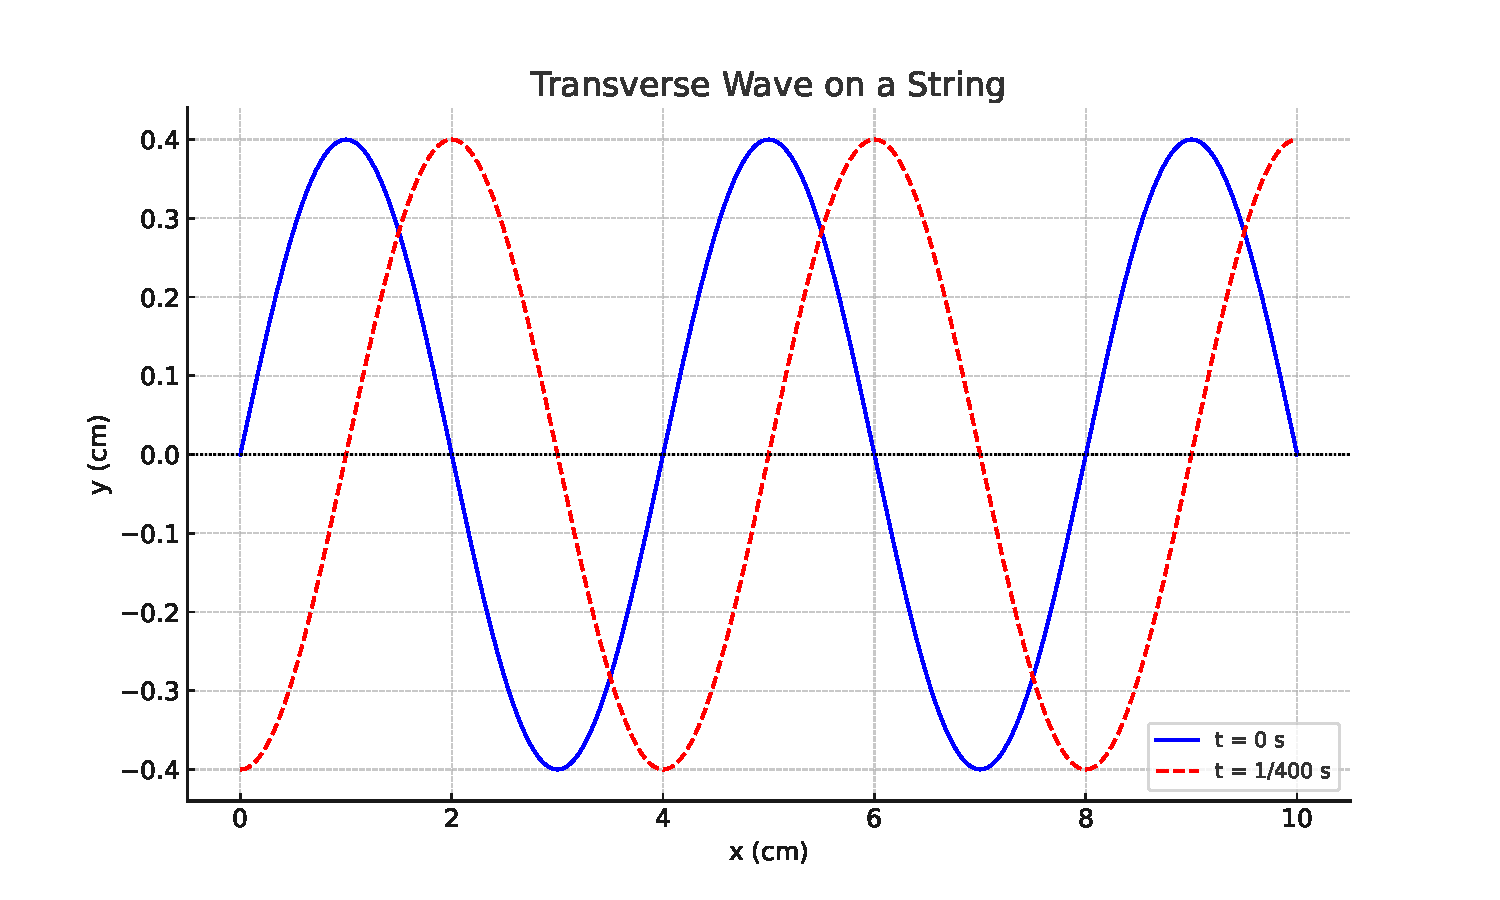
\includegraphics[width=1\linewidth]{figs/fig_sol_8.2b.pdf}
    %\caption{Caption}
    %\label{fig:enter-label}
\end{figure}
\\\textbf{Solution(c)}
\\
\\The transverse speed of any point on a transverse wave is given by
\[v_y=\frac{\partial y}{\partial t}=-80\pi\cos[\pi(0.5x-200t)]\]
$v_y$ is maximum when the cosine function is equal to $\pm1$. 
\[v_{y,\text{ max}}=80\pi\approx251\,\text{cm\,s}^{-1}.\]
\textbf{Solution(d)}
\\
\\For constant wavelengths of 4\,cm, we can have the first, second, third, and fourth harmonics. As the length $L$ is equal to $\frac{n\lambda}{2}$ (where $n=1,2,3,4,$ . . .) . Hence, the values of $L$ for this specific case are 2, 4, 6, and 8\,cm.

\subsubsection*{Problem 8.3 - Standing waves on a string}
The equation of a transverse standing wave on a string is given by $y=0.3(\sin3x)(\cos1200t)$ where $y$ and $x$ are in cm and $t$ in seconds.
\begin{enumerate}
    \item[(a)]What is the wavelength, wave number, frequency, and period of this wave?
    \item[(b)]Carefully draw the wave ($y$ versus $x$) at $t=0$, at $t=1.31\times10^{-3}\,$ s, and at $t=2.62\times10^{-3}\,$ s.
    \item[(c)]What is the maximum transverse speed?
    \item[(d)]What is the speed of propagation (of a transverse disturbance) \textit{along} the string?
\end{enumerate}
\textbf{Solution(a)}
\\
\\A traveling wave can be modeled by the function
\begin{equation}
    y(x,t)=A\sin kx\cos\omega t,
\end{equation}
which follows the same analogy as discussed in problem 8.4 for the quantities $A$, $k$, and $\omega$. Therefore, for the values given, 
\[k=3\,\text{cm}^{-1},\,\,\,\,\,\,\,\,\,\,\lambda=\frac{2\pi}{k}\approx2.1\,\text{cm},\,\,\,\,\,\,\,\,\,\,\,\omega=1200\,\text{rad\,s}^{-1},\]
\[f=\frac{\omega}{2\pi}\approx191\,\text{Hz},\,\,\,\,\,\text{and}\,\,\,\,\,T=\frac{2\pi}{\omega}\approx5.24\times10^{-3}\,\text{s}.\]
\textbf{Solution(b)}
\begin{figure}[h]
    \centering
    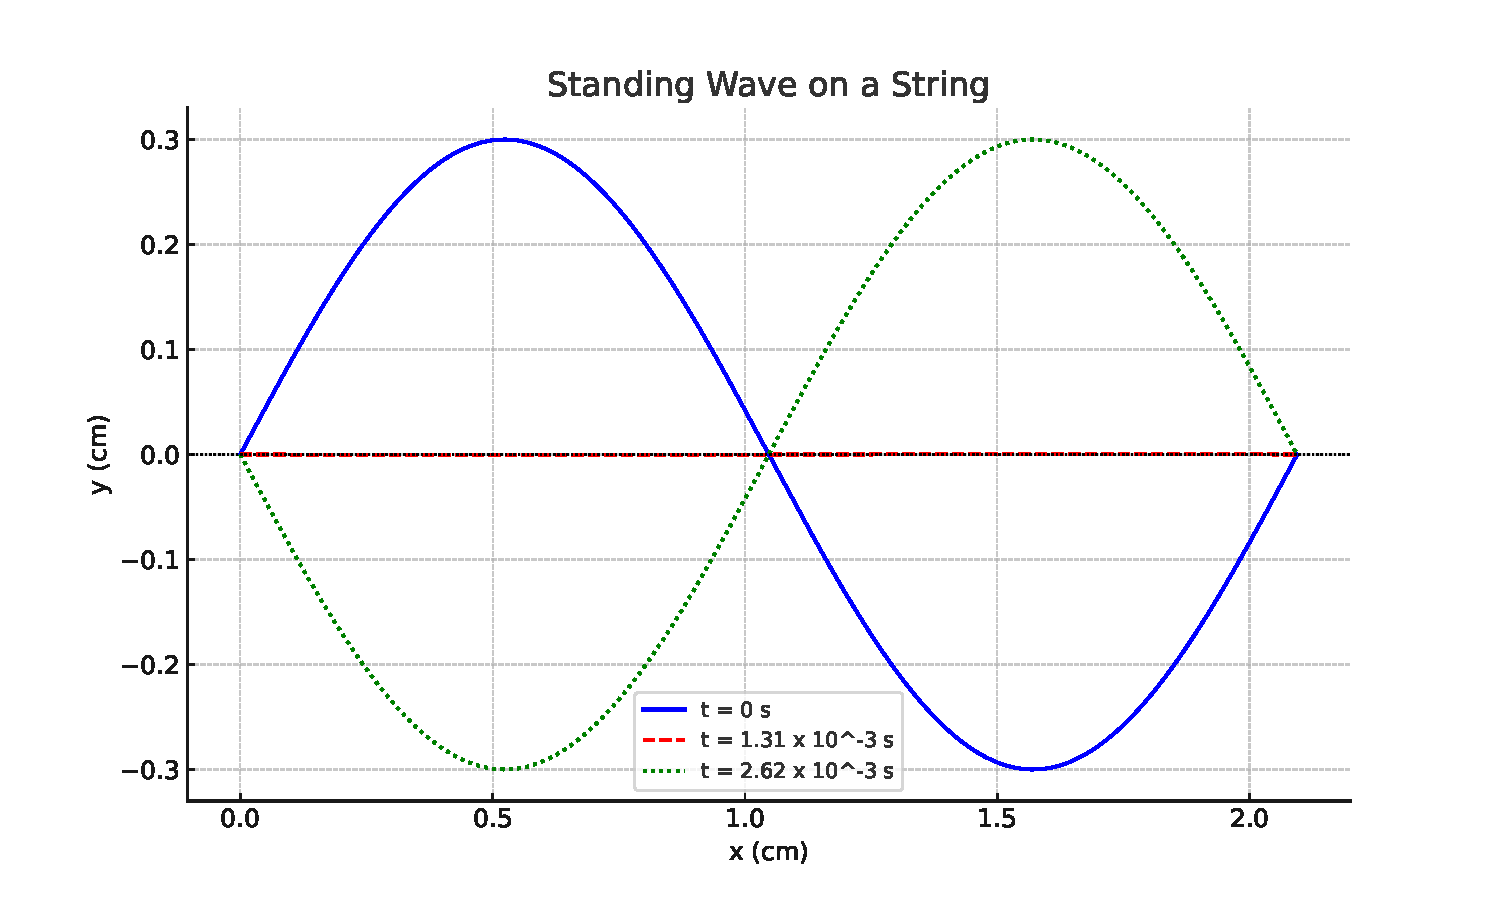
\includegraphics[width=0.95\linewidth]{figs/fig_sol_8.3b.pdf}
   % \caption{Caption}
   % \label{fig:enter-label}
\end{figure}
\\\textbf{Solution(c)}
\\
\\Again, using the same approach as in problem 8.2 (c), the transverse speed is \[v_y=\frac{\partial y}{\partial t}=-360\sin3x\sin1200t,\] that has a maximum value of 360\,cm\,s$^{-1}$.
\\
\\\textbf{Solution(d)}
\\
\\The phase speed is $\frac{\omega}{k}\approx400\text{cm\,s}^{-1}$. However, it is important to note that this speed does not mean that the waveforms are traveling at this speed; since this is a standing wave, the waveforms have zero speed because they are merely changing their phase with the passage of time.

\subsubsection*{Problem 8.4 - Average dissipated in an $LRC$ circuit}
In an $LRC$ circuit, suppose $I=I_0\sin\omega t$ and $V=V_0\sin(\omega t+\phi)$. Determine the instantaneous power
dissipated in the circuit from $P=IV$ using the equations and show that on average, $\bar{P}=\frac{1}{2}V_0I_0\cos\phi$
\\
\\\textbf{Solution}
\\
\\Using the expressions given for $I$ and $V$, we have
\[P=I_0V_0\sin\omega t\sin(\omega t+\phi)=I_0V_0\left(\sin^2\omega t\cos\phi+\sin\omega t\cos\omega t\sin\phi\right).\]
For the average power, we use the mean values of the functions $\sin^2\omega t$ and $\sin\omega t\cos\omega t$ over one period (which is $\frac{1}{2}$ and 0 respectively). Hence, on average,
\begin{equation}
    \bar{P}=\frac{1}{2}I_0V_0\cos\phi.
\end{equation}

\subsubsection*{Problem 8.5 - Width of resonance peak}
\begin{enumerate}
    \item[(a)]Determine a formula for the average power $\bar{P}$, dissipated in an $LRC$ circuit in terms of $L$, $R$, $C$, $\omega$, and $V_0$.
    \item[(b)]At what frequency is the power a maximum?
    \item[(c)]Find an approximate formula for the width of the resonance peak in average power, $\Delta\omega$, which is the difference in the two (angular) frequencies where $\bar{P}$ has half its maximum value. Assume a sharp peak.
\end{enumerate}
\textbf{Solution(a)}
\\
\\In an $RLC$ circuit, the phase angle is given by 
\begin{equation}
    \tan\phi=\frac{\omega L-\frac{1}{\omega C}}{R}.
\end{equation}
Thus, using the Pythagorean theorem on Eq. (6) gives
\begin{equation}
    \cos\phi=\frac{R}{\sqrt{R^2+\left(\omega L-\frac{1}{\omega C}\right)^2}}.
\end{equation}
Substituting equations 1 and 7 into Eq. (5) results in
\begin{equation}
    \bar{P}=\frac{V_0^2R}{2\left[R^2+\left(\omega L-\frac{1}{\omega C}\right)^2\right]}.
\end{equation}
\textbf{Solution(b)}
\\
\\The power is maximum when the terms $\omega L$ and $\frac{1}{\omega C}$ cancel each other, that is, when the inductive ($X_L$) and the capacitive ($X_C$) reactances are equal to each other.
\[X_L=X_C\Rightarrow\omega L=\frac{1}{\omega C}\Rightarrow\omega=\frac{1}{\sqrt{LC}}.\]
Thus the frequency for which the power is maximum is
\begin{equation}
    f=\frac{1}{2\pi\sqrt{LC}}.
\end{equation}
\\
\\
\textbf{Solution(c)}
\\
\\At the frequency given by Eq. (9), the maximum average power is $\bar{P}=\frac{V_0^2}{2R}$.
Thus, equating half the maximum power with Eq. (8) gives
\[\frac{V_0^2}{4R}=\frac{V_0^2R}{2\left[R^2+\left(\omega L-\frac{1}{\omega C}\right)^2\right]}\Rightarrow\omega L-\frac{1}{\omega C}=\pm R.\]
For a sharp resonance peak,
\begin{equation}
    \omega\approx\omega_0+\delta\omega.
\end{equation}
Substituting this value of $\omega$ into the relation we derived above gives
\begin{equation}
    (\omega_0+\delta\omega)L-\frac{1}{(\omega_0+\delta\omega)C}=\pm R
\end{equation}
where,
\[\frac{1}{(\omega_0+\delta\omega)C}\approx\frac{1}{\omega_0C}-\frac{\delta\omega}{\omega_0^2C}\]
is a good approximation. Given that $\omega_0L=\frac{1}{\omega_0C}$ and hence $L=\frac{1}{\omega_0^2C}$ (see part b). Now, Eq. (11) simplifies to
\[\omega_0L+\delta\omega L-\frac{1}{\omega_0C}+\frac{\delta\omega}{\omega_0^2C}=\pm R\Rightarrow\delta\omega=\pm\frac{R}{2L}.\]
Eq. (10) now gives two frequencies at which the average power is half of its maximum value.
\[\omega_-=\omega_0-\frac{R}{2L}\,\,\,\,\,\text{and}\,\,\,\,\,\omega_+=\omega_0+\frac{R}{2L}.\]
Finally, width of the resoncance peak is given by
\[\Delta\omega=\omega_+-\omega_-=\frac{R}{L}.\]





\subsubsection*{Problem 8.6 - Distance sensing with sound}
A bat can sense its distance from the wall of a cave (or whatever) by emitting a sharp ultrasonic pulse that reflects off the wall. The bat can tell the distance from the time the echo takes to return.
\begin{enumerate}
    \item[(a)]If a bat is to determine the distance to a wall $8\,$m away with an error of less than $\pm0.2\,$m, how accurately must it sense the time interval between emission and return of the pulse?
    \item[(b)]Suppose that a bat flies into a cave filled with methane (swamp gas). By what factor will this gas distort the bat's perception of distances? At 20°\,C, the speed of sound in methane is 432\,m/s.
\end{enumerate}
\textbf{Solution(a)}
\\
\\Time between the emission and detection of the reflected pulse from the wall is given by $T=\frac{2L}{v}$, where $L$ is the distance between the bat and wall and $v$ is the speed of sound in air at standard conditions and has a value of 343\,ms$^{-1}$. Thus, the maximum error that bat can afford in the value of time is
\[\Delta T=\frac{2\Delta l}{v}\approx1.2\times10^{-3}\,\text{s}.\]
\textbf{Solution(b)}
\\
\\Due to the presence of methane, the bat will receive the reflected signal more quickly, and therefore the perceived distance $L_{\text{apparent}}$ would be smaller than the actual distance $L_{\text{real}}$. For example, the perceived distance is
\[L_{\text{apparent}}=\frac{v_aT}{2}=\frac{v_a}{v_m}L_{\text{real}}\]
where $v_a$ is speed sound in air, $v_m$ is speed of sound in methane, and $T$ is the actual time between emission and reflection ($T=2L_{\text{real}}/v_m$). Substituting the values gives
\[L_{\text{apparent}}=0.8L_{\text{real}}.\]
Bat will interpret the actual distance to be 20\% less than its true value.

\end{document}
